\section{structure}

Creating actual rather than virtual interdisciplinary centres is likely to improve the chances of interdisciplinary research and teaching lasting. The following subsections discuss the answers obtained for each specific question.


\subsection{Interdisciplinary centres}

\begin{figure}[h]
\centering
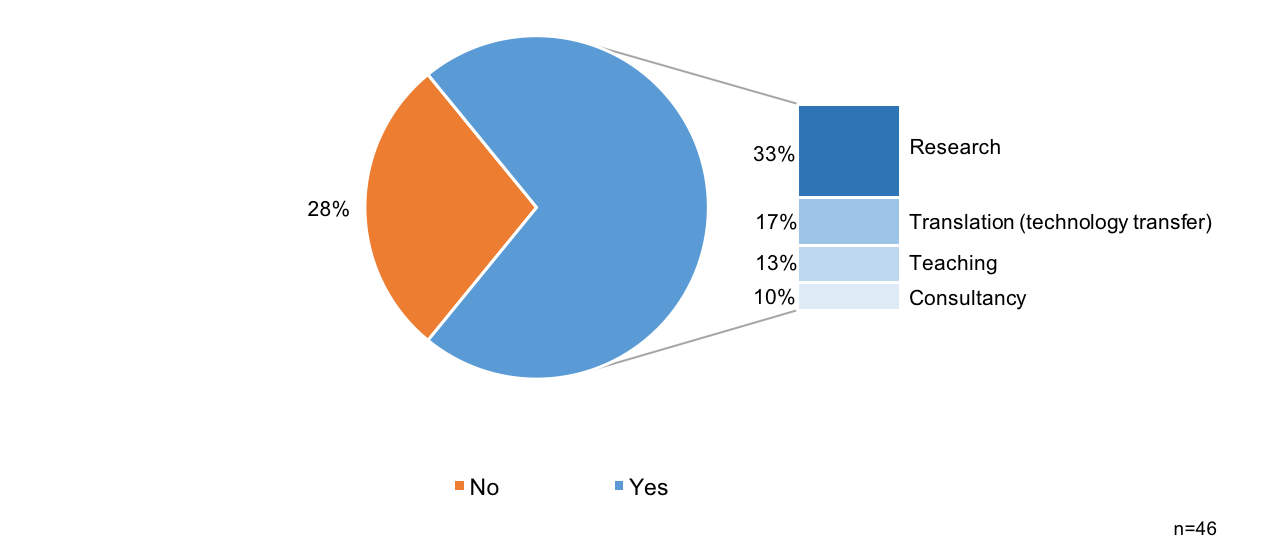
\includegraphics[width = \linewidth]{charts/5a.png}
\caption{Does your university set up centres for interdisciplinary work?}
\label{sect5:centres}
\end{figure}

28\% of respondents say their university does not have real interdisciplinary centres (see Figure~\ref{sect5:centres}). Of those who commented on why the lack of centres only one actually replied that their management was averse to setting up additional administrative structures. The rest just said there were informal groupings, but nothing officially supported. 45\% of all of the interdisciplinary centres are set up primarily for research and only 18\% for teaching. The rest are primarily involved with industry.

There are a broad range of centres in the different universities -- clearly what expertise is in a university and what the structure of the different departments/schools/faculties impacts which centres are set up in addition to the existing primary structures. The most common centres mentioned with a significant Informatics component are in Computational Science, Data Science,  Life Science, Digital Society, Energy, and Security.   There were also more than one university with the following centres: Biomedical Engineering, Environment/Climate,  Medical Imaging, and  Complex Systems. There are a wide range of centres which only mentioned at one university: Health,  FinTech, Digital Humanities, Robotic Surgery, Cognitive Ageing, Bioinformatics, and Geoinformatics, 
 


\subsection{Purpose of interdisiciplinary centres}

\begin{figure}[h]
\centering
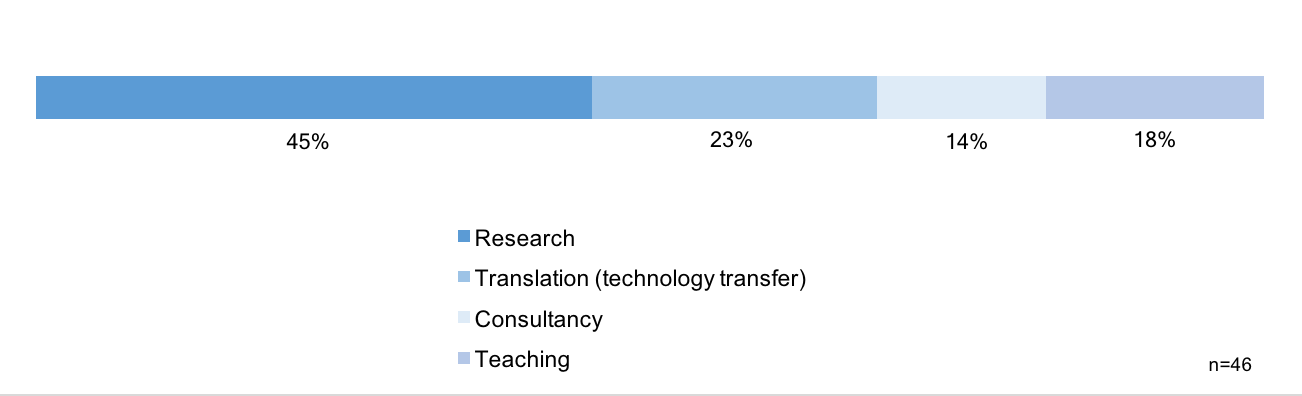
\includegraphics[width = \linewidth]{charts/5b.png}
\caption{Why were the centres created?}
\label{sect5:reasons}
\end{figure}

45\% of all of the interdisciplinary centres are set up primarily for research and only 18\% for teaching (see Figure~\ref{sect5:reasons}). The rest are primarily involved with industry collaboration or consultancy.

\subsection{ Ownership of interdisciplinary centres}

\begin{figure}[h]
\centering
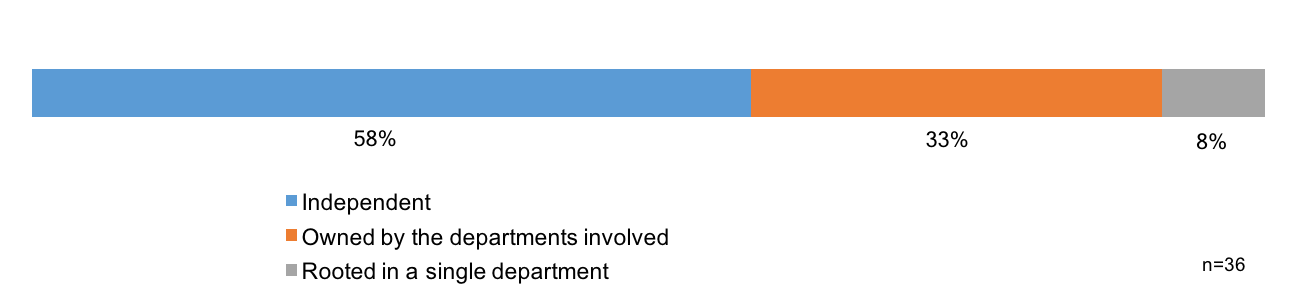
\includegraphics[width = \linewidth]{charts/5c.png}
\caption{Which entity control the interdisciplinary centres?}
\label{sect5:owners}
\end{figure}

Of the 36 respondents, 21 (or 58\%) are independent entities within their university, 12 (or 1/3) are co-owned by the departments that are involved and the rest have a single department that owns them (see Figure~\ref{sect5:owners}). It is surprising that so many are separate entities as this means if they are not self-funding money will be an issue.

\subsection{ Location of interdisciplinary centres}

\begin{figure}[h]
\centering
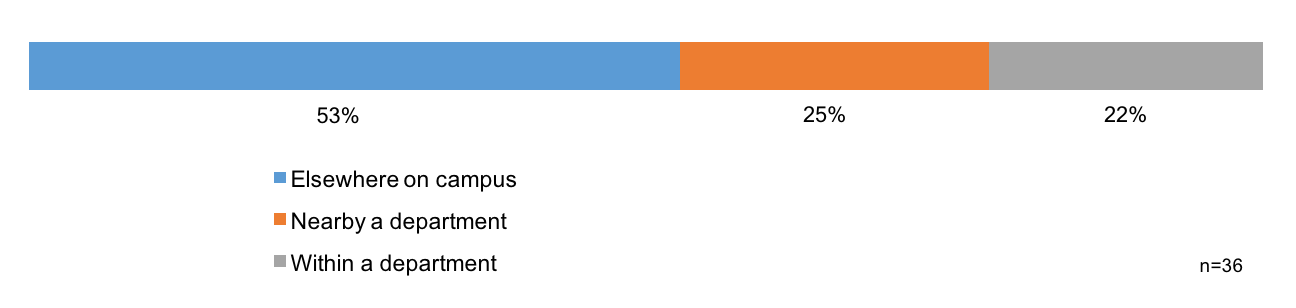
\includegraphics[width = \linewidth]{charts/5d.png}
\caption{ Where are the centres located?}
\label{sect5:locations}
\end{figure}

More than half of the respondents report that the centres they are reporting on are located `elsewhere' on campus (see Figure~\ref{sect5:locations}). although a significant minority described the centres as `virtual' implying that they actually had no physical location. One contributor distinguished between a large centre that had its own space, and smaller ones that were embedded in departments. Others spoke of large buildings that accommodated many different groups such that a nearby centre may not be associated with a department.

\subsection{Funding of interdisciplinary centres}

\begin{figure}[h]
\centering
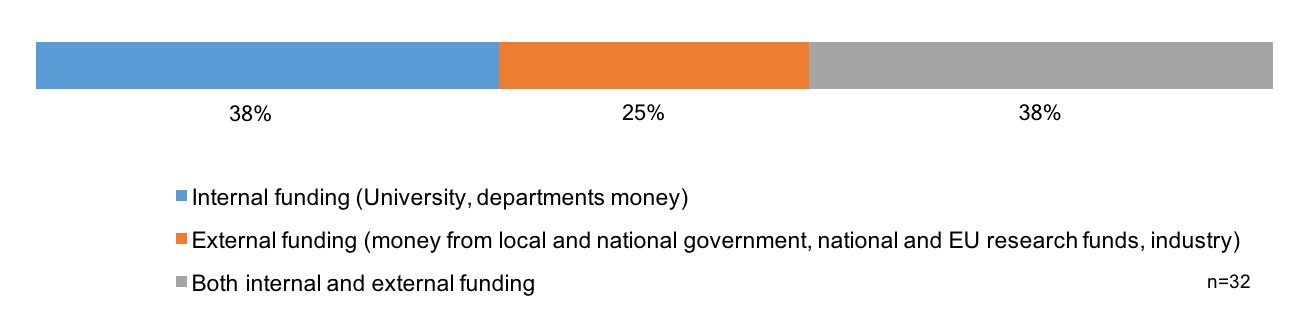
\includegraphics[width = \linewidth]{charts/5e.png}
\caption{Who funds interdisciplinary centres?}
\label{sect5:funding}
\end{figure}

Only 25\% of the interdisciplinary centres reported on are funded entirely externally, the funding of the rest being equally split between entirely internal and mixed sources of funding (see Figure~\ref{sect5:funding}). In the majority of cases where funding is entirely internal, the bulk of the actual cash seems to come from central funds with departments providing resources `in kind'. Frequently, time-limits are expressed (five and six years are mentioned) after which the centre is expected to be self-financing. For the universities that reported on (entirely or partially) external funding, in many cases only government and EU programmes were explicitly cited as sources of funds.

\subsection{Planning for changing interdisciplinary centres}

\begin{figure}[h]
\centering
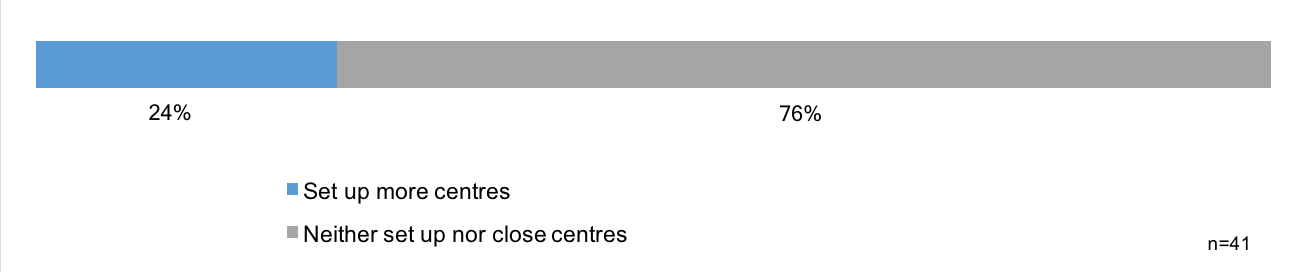
\includegraphics[width = \linewidth]{charts/5f.png}
\caption{Are there changes planned for setting up or closing centres?}
\label{sect5:changes}
\end{figure}

A quarter of respondents report on plans to set up new centres (see Figure~\ref{sect5:changes}). Some describe a notion of continuous evolution of interdisciplinary work. Only AI was explicitly mentioned as a target for the development of new centres. Other respondents, although not explicitly planning a new centre, mention the issue of the periodic review of existing centres citing various options including merging centres and/or creating new centres.  

\subsection{Drivers for new activities}

\begin{figure}[h]
\centering
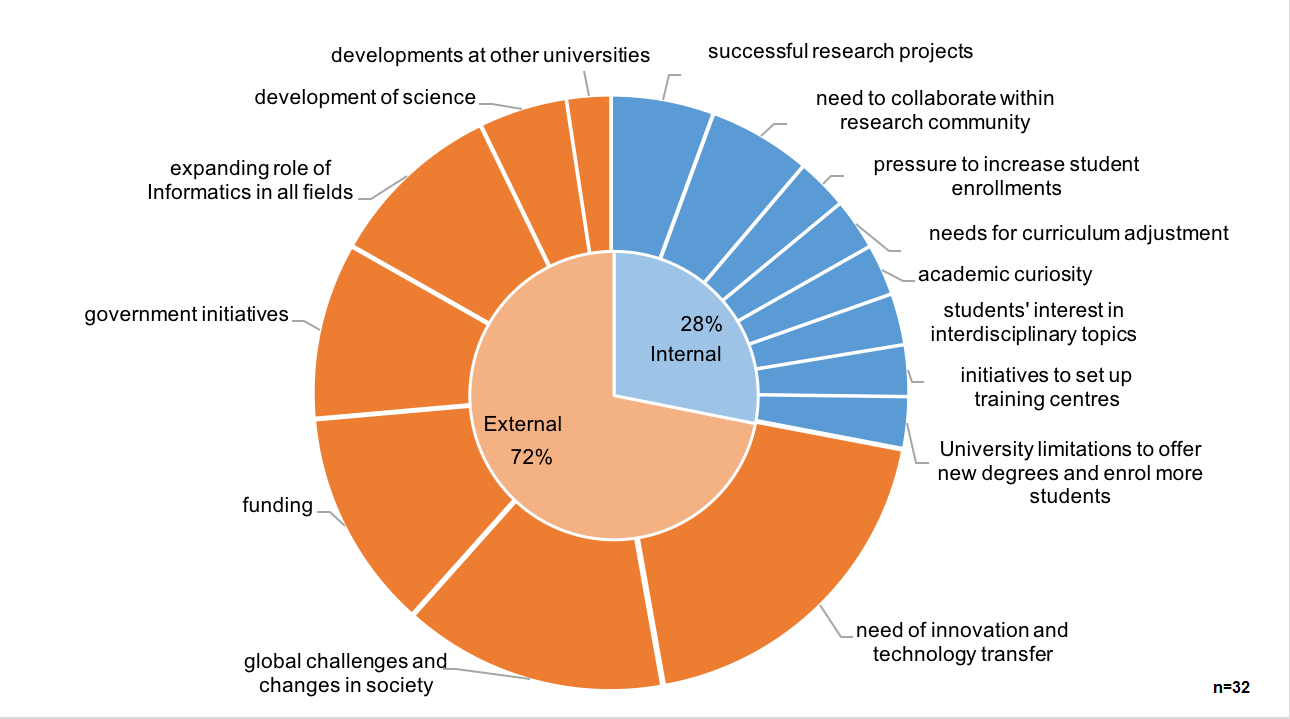
\includegraphics[width = \linewidth]{charts/5g.png}
\caption{What are the drivers and pressures for new centres?}
\label{sect5:drivers}
\end{figure}
                                                                                                                    
Nearly one third of respondents reported on internal drivers and pressures bearing on innovative activity (see Figure~\ref{sect5:drivers}). Amongst the drivers, academic curiosity of staff and students was cited alongside a need for research collaboration. Pressures included demands to increase students enrolment, to modify the curriculum and university initiatives to set up a centre. One university also mentioned limitations of student numbers and limitations on joint degrees that inhibited their development goals.

The other respondents addressed external drivers and pressures. The most significant cited pressure concerned the societal influence of globalisation together with an associated driver on universities to promote innovation and  technology transfer (47\%).  The next most significant pressure is the search for funding driven by government initiatives (30\%) whilst other respondents observed the expanding role of Informatics in other disciplines and the pressure on Informatics departments to support these disciplines (20\%). Finally, one respondent mentioned competition between universities as an external pressure.

\subsection{Support for interdisciplinary work}

\begin{figure}[h]
\centering
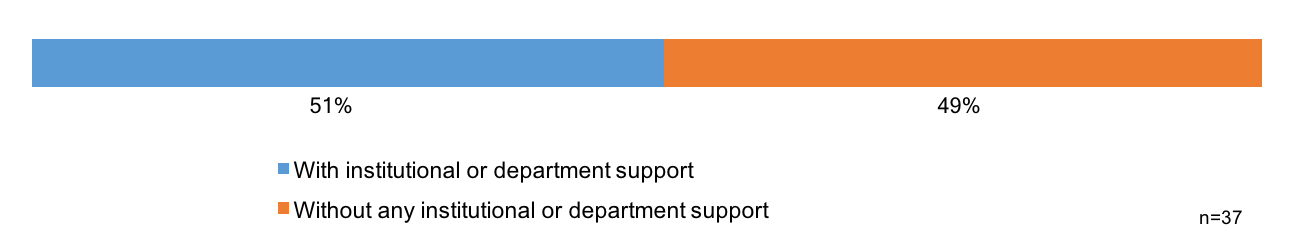
\includegraphics[width = \linewidth]{charts/5h.png}
\caption{Is any support provided for interdisciplinary work?}
\label{sect5:support}
\end{figure}

Respondents were evenly split over this question (see Figure~\ref{sect5:support}) although several of those who claimed institutional support were rather equivocal - "I would guess so" and ``Some departments \ldots ''. Respondents who reported no institutional support divided into those who stipulated some form of external support and those who did it ``as a hobby'' (~25\%).

\subsection{Strategic vision }
\begin{figure}[h]
\centering
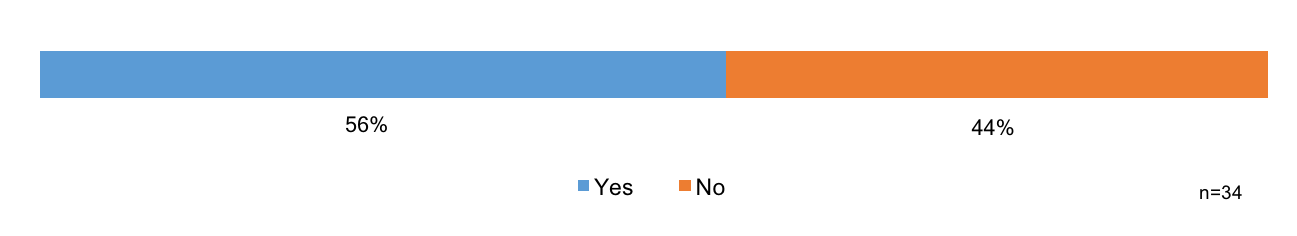
\includegraphics[width = \linewidth]{charts/5i.png}
\caption{Are there any centres for interdisciplinary work created from strategic initiatives?}
\label{sect5:strategy}
\end{figure}

More than half of the respondents reported on centres created from strategic initiatives (see Figure~\ref{sect5:strategy}). Many of these were oriented towards Informatics themes (FinTech, Crypto-currencies, Data Science) but several other types of centre were mentioned (Learning and Education, Cultural Heritage, Sustainability and Energy).

\subsection{Official strategic vision}
\begin{figure}[h]
\centering
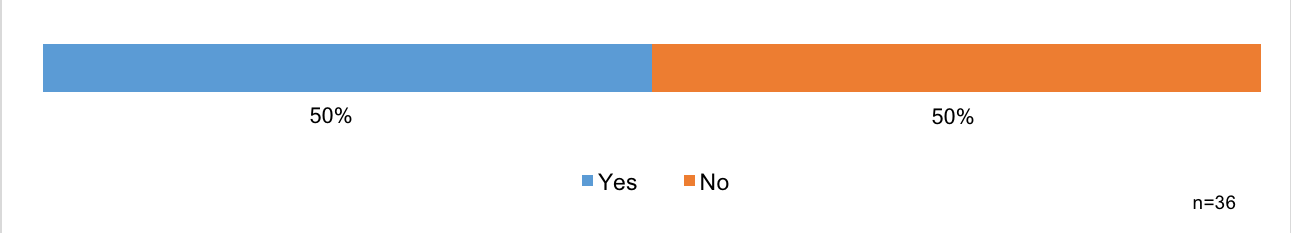
\includegraphics[width = \linewidth]{charts/5j.png}
\caption{Is there an official strategy to widen the role of Informatics?}
\label{sect5:official}
\end{figure}

Respondents were exactly split on this question (see Figure~\ref{sect5:official}). Of those who answered positively, the emphasis was on multidisciplinarity for about half the respondents. Informatics topics cited by others included Cyber Security, Data-driven Innovation, Intelligent Systems, Applied Computer Science and Digital Humanities. Respondents who answered ``No'' were not very forthcoming with their comments.

\subsection{Final thoughts}

Nineteen respondents contributed their overall views on the current situation in their universities. One response was wholeheartedly supportive citing good funding, strong collaboration and a sound international reputation as attractive to world-class researchers. Other commentators mentioned limited or non-existent funding and other, higher priorities (like increased student enrolment) as factors which retarded interdisciplinary initiatives. Two universities thought that Informatics was too junior a partner in the context of their university to make much impact.

By far the most significant issue concerned the nature of either the central or departmental strategic direction. Three respondents asked for greater freedom for individual researchers to be more creative with ideas, contacts and funding.  However, there were ten contributors who asked for better communication between faculties, more structured research management or further internationalisation. A few just wanted more substance to the strategy - ``It is only a goal without supporting instruments. '';  ``Still under construction - too early to conclude \ldots ''.




